\section{Experiments}\label{sec:experiments}
\subsection{Experimental setup}\label{sec:exp_setup}
We evaluate posterior accuracy, stability and measured computational efficiency separately. Table~\ref{tab:exp_overview} lists the experiment families, the question each addresses and its protocol status; the labels P1--P4 used below refer to that table. The main nonquadratic targets are Bayesian logistic regressions with Gaussian priors. German Credit has $N=1{,}000$ and $d=61$ after the frozen encoding; Bank Marketing uses all $45{,}211$ observations of \texttt{bank-full.csv}, with $d=43$ after encoding \citep{hofmann1994german,moro2014bank}. Bank's duration variable is retained: this is a posterior-sampling benchmark, not a prospective prediction exercise. Four fixed-size synthetic targets have $N=30{,}000,d=20$ and differ in feature geometry and signal. Additional synthetic targets vary $N$ while holding the data-generating mechanism fixed.
\begin{table}[tb]
\centering\footnotesize
\caption{Experiment families, the question each addresses and its protocol status. Labels P1--P4 are used throughout Section~\ref{sec:experiments} and Appendix~\ref{app:protocols}.}\label{tab:exp_overview}
\setlength{\tabcolsep}{3pt}
\begin{tabular}{@{}>{\raggedright\arraybackslash}p{0.11\linewidth}>{\raggedright\arraybackslash}p{0.23\linewidth}>{\raggedright\arraybackslash}p{0.24\linewidth}>{\raggedright\arraybackslash}p{0.25\linewidth}>{\raggedright\arraybackslash}p{0.09\linewidth}@{}}
\toprule
Study & Target & Question & Protocol status & Section \\
\midrule
P1 & German Credit ($N=1{,}000$, $d=61$) & Matched-step accuracy of CV1, CV2 and ULA; cost of CV2 & Frozen held-out primary criterion; frozen A100 replication & \ref{sec:exp_accuracy} \\
\addlinespace[5pt]
P2 & Four synthetic logistic targets ($N=30{,}000$, $d=20$); original Bank ($N=45{,}211$, $d=43$) & Fixed-budget accuracy at selected steps & Frozen held-out primary criteria (synthetic); frozen selected-step held-out comparison (Bank) & \ref{sec:exp_accuracy} \\
\addlinespace[5pt]
P3A & Bank: original-target tuning and failure analysis; $\log(1+\texttt{previous})$ target & Stability mechanism; optimized time-to-accuracy & Exploratory extension designed after the original Bank results; separate pilot and validation seeds within each stage & \ref{sec:exp_bank} \\
\addlinespace[5pt]
P3B & Nested AR(1) synthetic logistic ($d=20$, $N=2{,}000$--$128{,}000$) & Gradient-noise and time-to-accuracy scaling in $N$; full-gradient ULA comparison & Frozen before new observations and outcomes; ULA comparison is a review-motivated two-stage extension & \ref{sec:exp_scaling} \\
\addlinespace[5pt]
ESS & German selection seeds; YearMSD & Post-burn-in mixing per unit cost & Descriptive, from existing chain records & \ref{sec:exp_ess} \\
\addlinespace[5pt]
P4 & Quadratic Gaussian ($N=256$, $d=10$, $\kappa\in\{10,10^4\}$) & Numerical exactness; geometry versus discretization & Verification with fixed tolerances; no performance search & \ref{sec:exp_gaussian} \\
\addlinespace[5pt]
YearMSD & Gaussian ridge regression ($N=463{,}715$, $d=90$) & Geometry under near-exact gradients & Historical, chain-based evaluation & \ref{app:year_geometry} \\
\bottomrule
\end{tabular}
\end{table}


Unless explicitly labelled as a Gaussian ablation, preconditioning means
\begin{equation}\label{eq:exp_metric}
 P=\{H(\hat\theta)+\lambda I\}^{-1},\qquad H(\hat\theta)=\nabla^2U(\hat\theta),
\end{equation}
held fixed during sampling. The numerical ridge is $\lambda=10^{-10}$ in the principal logistic studies; the prior curvature is already part of $H$. This metric Hessian differs from the likelihood Hessian in the control-variate estimator. Both CV1 and CV2 require the metric construction in this framework. We use
\begin{equation}\label{eq:exp_update}
 \theta_{k+1}=\theta_k-hP\widehat{\nabla U}(\theta_k)+\sqrt{2h}\,L\zeta_{k+1},
 \qquad LL^\top=P,\quad\zeta_{k+1}\sim N(0,I),
\end{equation}
with the injected-noise notation of~\eqref{eq:sgld}. Step grids are scaled by $L_P=\lambda_{\max}(P^{1/2}HP^{1/2})$. Statements about the identity-coordinate analysis above are not used as an unqualified guarantee for these measured fixed-metric comparisons. Adaptive preconditioners are outside the scope of the primary comparisons (Section~\ref{sec:related}).

Each ensemble contains independent replicas initialized at the mode. Main held-out/validation comparisons use $R=512$ replicas and eight algorithm seeds; method pairing is preserved within each experiment. At iteration $K$, one endpoint from each replica estimates the marginal law of the iterate. We do not pool successive states to estimate that marginal law. Separate ergodic functionals estimate posterior variances. Full-gradient ULA uses the same metric as a stochastic-gradient-noise control and retains discretization error.

For logistic targets, we compare endpoints with two independently constructed full-data HMC reference pools. References must pass frozen rank-$\widehat R$, bulk/tail ESS, acceptance, divergence and between-pool agreement gates before posterior rankings are used (Appendix~\ref{app:references}).

The principal transport metric is sliced $W_2$ (SW$_2$) in declared posterior-standardized coordinates. The other principal metric is relative posterior-variance NRMSE. These measure different objects and can rank methods differently. German's original variance criterion used a reference-calibration normalization; it is not numerically interchangeable with later relative NRMSE. Appendix~\ref{app:metrics} defines both and preserves the exploratory harmonized analysis.

Runtime is setup-inclusive wall-clock for an entire replica ensemble. Required anchor fitting, Hessian construction, inverse/factorization, estimator caches and synchronized sampling are included under each study's declared attribution. Warm timings reuse compiled code but start fresh replicas; cold timings additionally include recorded compilation attribution. Reference generation, scoring and reporting are separate research costs. Search-inclusive costs are distinguished from selected-configuration costs. JAX \citep{jax2018github} uses float64 in the principal migrated studies. Section~\ref{sec:exp_limitations} collects the scope conditions that apply to all of these comparisons.

\subsection{Sampling accuracy at frozen selections (P1 and P2)}\label{sec:exp_accuracy}
The German CPU held-out experiment and frozen A100 replication each contain $120$ runs; respectively three and nine failed replicas are retained. Both detect a material CV1--ULA accuracy gap. However, the original joint criterion, SW$_2\leq0.113$ and native variance NRMSE$\leq0.1$, does not conservatively establish CV2 efficiency: held-out means pass while accuracy upper intervals do not. A favorable marginal timing comparison cannot replace this joint outcome. In the GPU variance-only analysis, the warm CV2/CV1 cost ratio is approximately $0.284$, but this is exploratory and uses the native German normalization. The replication reuses frozen CPU choices, rather than searching for GPU-optimal configurations.

Original Bank gives a different limitation. At $K=2048$, CV2 reduces SW$_2$ from $0.689$ to $0.188$ and variance NRMSE from $1.501$ to $0.838$ relative to CV1, but increases warm time from $1.338$ to $1.828$ seconds. The paired SW$_2$ difference is $-0.501$ (95\% interval $[-0.639,-0.376]$); the variance difference is $-0.663$ ($[-1.030,-0.035]$). Neither CV method reaches the frozen joint target SW$_2\leq0.3$, variance NRMSE$\leq0.5$ at any tested checkpoint through $8192$ on both reference means; ULA does. These selected-step results do not establish a CV1/CV2 time-to-target advantage. They also show that absence of a numerical failure does not imply acceptable posterior accuracy.

On the four fixed-size synthetic targets, CV2 improves the prespecified $K=2048$ variance outcome in all regimes (Table~\ref{tab:p2_synthetic}). All four adjusted intervals exclude zero. CV2 closely tracks ULA, but its warm time at this fixed budget is about $1.4$--$2.1\%$ above CV1. SW$_2$ does not improve uniformly: in the correlated strong-signal regime it is $0.1480$ for CV2 versus $0.1475$ for CV1. Moreover, every method already meets the original loose joint target at the earliest checkpoint $K=128$. That target therefore cannot distinguish an iteration advantage. Later threshold sensitivity is reported as exploratory, not substituted for the original primary criterion. In summary, P2 shows accuracy improvements of CV2 over CV1 at selected steps, chiefly in variance estimation, while neither P1 nor P2 establishes an efficiency advantage under its prespecified criterion.
\begin{table}[tb]
\centering\small
\caption{Prespecified synthetic variance outcomes at $K=2048$ (primary reference). Differences are CV2 minus CV1; intervals use the four-contrast Bonferroni adjustment.}\label{tab:p2_synthetic}
\begin{tabular}{lrrrr}
\toprule
Regime & CV1 & CV2 & Difference & 98.75\% interval \\
\midrule
Correlated, signal 1 & 0.1535 & 0.1390 & -0.0145 & $[-0.0148,-0.0143]$ \\
Scaled, signal 1 & 0.1750 & 0.1572 & -0.0178 & $[-0.0180,-0.0174]$ \\
Correlated, signal 3 & 0.1832 & 0.1590 & -0.0242 & $[-0.0247,-0.0236]$ \\
Benign, signal 1 & 0.1647 & 0.1414 & -0.0234 & $[-0.0238,-0.0230]$ \\
\bottomrule
\end{tabular}
\end{table}


\subsection{Stability and computational efficiency on Bank (P3A)}\label{sec:exp_bank}
Apart from the frozen selected-step comparison in Section~\ref{sec:exp_accuracy}, every Bank analysis below belongs to the exploratory P3A extension. These stages were designed after the original Bank results. Each stage separates its pilot and validation seeds prospectively, but the feature transformation and the tuning search were both introduced after the original failures were observed, so their separate contributions to the final improvement cannot be identified from the final ratio alone.

\paragraph{Original-target failure and implementation checks.}
Batch-size optimization on original Bank initially gives an unfavorable CV2 frontier. After a bounded small-step extension on JAX CPU, $296$ validation runs contain $28$ failed replicas in $20$ runs, all CV2. CV1 has $18/18$ stable candidate configurations, compared with $8/16$ for CV2 through the complete horizon. At relative variance thresholds $0.5$, $0.4$ and $0.3$ with SW$_2\leq0.3$, CV1's descriptive warm minima are several times smaller than CV2's (Table~\ref{tab:bank_original_minima}); at $0.2$, CV2 does not reach the target in the tested budget. Some point-attainment cells have borderline accuracy uncertainty.
\begin{table}[tb]
\centering\small
\caption{Original Bank after the bounded small-step extension (P3A): descriptive setup-inclusive warm minima, in seconds, for joint targets with SW$_2\leq0.3$.}\label{tab:bank_original_minima}
\begin{tabular}{rrr}
\toprule
Variance threshold & CV1 & CV2 \\
\midrule
0.5 & 5.26 & 34.5 \\
0.4 & 8.44 & 44.3 \\
0.3 & 19.9 & 176 \\
\bottomrule
\end{tabular}
\par\smallskip{\footnotesize At threshold $0.2$, CV2 does not reach the target within the tested budget.}
\end{table}


An implementation audit passes $306$ fixed-input NumPy/JAX checks of gradients, corrections and updates, and reconciles the recorded costs. Exact finite-population noise calculations at common posterior locations reveal substantial heterogeneity. CV2 has lower preconditioned noise at $14/16$ reference locations, with median CV2/CV1 ratio $0.020$ but ratio of means $0.594$ and maximum ratio $7.12$. A low median is thus not evidence of a comparably large expected-noise reduction. Modest minibatch Monte Carlo probes can miss the rare observation contributions captured by exact enumeration.

\paragraph{Observation-level intervention.}
Original-stream replay identifies large stochastic drift, rather than the injected Gaussian increment, in the tested terminal updates. Observation $29182$, with standardized \texttt{previous} approximately $119$, occurs in $27/28$ failed-replica triggering batches and $19/20$ first-failure batches. At fixed pre-failure states and random inputs, replacing this observation prevents overflow in $304/304$ single-step proposals. Sham replacement of an ordinary observation while retaining it leaves $208/208$ proposals overflowing. These are controlled one-step interventions, not estimates of long-run effects of deleting a datum. Shared random streams across step configurations also make the event counts dependent. The original dataset and all failures are retained.

\paragraph{Feature sensitivity and optimized comparison.}
We next declare two exploratory feature transformations: $\log(1+\texttt{previous})$ and winsorization at the fixed $99.9\%$ quantile, followed by standardization of that column. Each defines a different posterior and receives a newly fitted mode, metric and reference. At matched whitened radius $\sqrt d$, median maximum CV2 remainder norms are approximately $0.048$ times their original values under either transformation, while posterior Hessian condition numbers remain similar (approximately $581$--$589$). Observation-level remainder risk therefore carries information beyond global conditioning in this comparison.

Small fixed-configuration studies recover an accuracy benefit but do not settle optimized efficiency. We consequently conduct one bounded, symmetric search on the log-transformed target over minibatch sizes $\{1,4,16,32,64,256\}$, locally scaled steps and checkpoint budgets. The $192$-run pilot freezes $24$ candidate configurations before $192$ independent validation runs. Each validation run has $512$ replicas and horizon $4096$. Sixteen runs contain $54$ failed replicas, all in three aggressive CV2 configurations; these complete configurations are excluded at every checkpoint rather than scoring survivors or their earlier prefixes.

Figure~\ref{fig:log1p_frontier} (top row) displays the validated accuracy--cost frontier over the tested configurations. It retains every eligible point and identifies the non-dominated boundary separately for each method and accuracy metric. A point lies on a boundary if no tested point for that method has both no greater time and no greater error, with at least one strict improvement. These two-dimensional frontiers characterize the tradeoff after tuning $n,h,K$; they are not continuous-parameter optima. In particular, a marginal SW$_2$ or variance frontier alone does not establish joint attainment of both accuracy requirements.

We therefore also report the joint time-to-accuracy function
\begin{equation}\label{eq:exp_joint_time}
 T_m(\varepsilon)=\min_{(n,h,K)\in\mathcal G_m^{\mathrm{valid}}}
 \left\{\overline T_m(n,h,K):
 \begin{aligned}
  \mathrm{SW}_2(n,h,K)&\leq0.3,\\
  E_{\mathrm{var}}(n,h,K)&\leq\varepsilon
 \end{aligned}\right\},
\end{equation}
where $\mathcal G_m^{\mathrm{valid}}$ is the frozen candidate/checkpoint grid that passes the complete validation-horizon failure rule. For point attainment, both inequalities use the worse of the two reference means. Supported attainment replaces each accuracy mean by its simultaneous upper bound. Time is setup-inclusive warm wall-clock unless explicitly labelled cold. An unattained target is reported as Not Reached, without a finite or infinite speedup. The SW$_2$ requirement rarely binds: it excludes $5$ of $84$ eligible CV1 configuration/checkpoints and $1$ of $63$ for CV2, so joint attainment is determined mainly by the variance tolerance.

The joint curve favors CV2 across all $41$ tested warm thresholds in both the point and supported analyses, whose selected configurations can differ (Figure~\ref{fig:log1p_joint}, bottom row). Representative joint targets yield warm speedups $2.27$--$6.27$ and cold speedups $1.35$--$4.07$ (Table~\ref{tab:log1p_speedup}). At variance target $0.3$, CV1 takes $3.08$ seconds and CV2 $0.491$, with speedup $6.27$ and approximate 95\% interval $[4.28,6.30]$. CV2's selected configuration uses the earliest validated checkpoint, $K=128$, at $24$ of the $41$ warm thresholds, compared with $10$ for CV1; at those thresholds the checkpoint grid, rather than further accuracy, limits the attainable CV2 time. Taken together, P3A identifies rare high-leverage Taylor remainders as a failure mechanism on original Bank, and shows a validated CV2 time-to-accuracy advantage on a transformed posterior, without separating the contributions of transformation and tuning.
\begin{table}[tb]
\centering\small
\caption{Optimized log-transformed Bank: setup-inclusive point-attainment times and speedups. Both reference accuracy means must satisfy SW$_2\leq0.3$ and the variance threshold.}\label{tab:log1p_speedup}
\begin{tabular}{rrrrrr}
\toprule
Variance & CV1 s & CV2 s & Warm ratio & 95\% interval & Cold ratio \\
\midrule
0.50 & 0.456 & 0.201 & 2.270 & $[2.259,2.281]$ & 1.348 \\
0.40 & 1.093 & 0.287 & 3.810 & $[3.785,3.830]$ & 2.240 \\
0.30 & 3.080 & 0.491 & 6.272 & $[4.284,6.296]$ & 3.976 \\
0.20 & 8.154 & 1.727 & 4.723 & $[4.710,4.736]$ & 4.070 \\
\bottomrule
\end{tabular}
\par\smallskip{\footnotesize Ratios are CV1/CV2. Intervals are approximate paired-seed bootstrap intervals that reselect the eligible minimum in each resample (Appendix~\ref{app:selection}).}
\end{table}

\begin{figure}[p]
\centering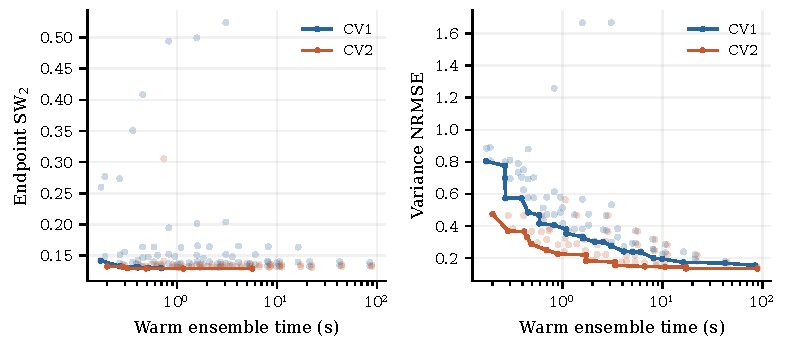
\includegraphics[width=\linewidth]{figures/log1p_frontiers.pdf}
\par\smallskip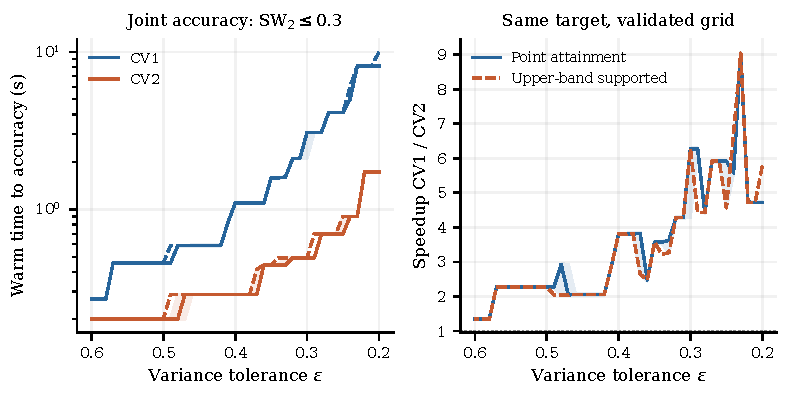
\includegraphics[width=\linewidth]{figures/log1p_joint_tta.pdf}
\caption{Validated accuracy--cost results for log-transformed Bank (P3A). Top: marginal SW$_2$ and variance-NRMSE frontiers against setup-inclusive warm JAX CPU ensemble time; faint points are all eligible $(n,h,K)$ configurations and lines the non-dominated boundaries. Bottom: joint time-to-accuracy (left) and CV1/CV2 speedup (right) with SW$_2\leq0.3$, across $41$ variance tolerances. Solid curves use point attainment and dashed curves supported attainment; shading gives approximate pointwise 95\% paired-bootstrap intervals.}\label{fig:log1p_frontier}\label{fig:log1p_joint}
\end{figure}
\FloatBarrier

\subsection{Dataset-size scaling (P3B)}\label{sec:exp_scaling}
We generate nested Bayesian logistic datasets with $d=20$, Gaussian features having AR(1) covariance $\Sigma_{ij}=0.5^{|i-j|}$, fixed alternating-sign coefficients scaled to population logit standard deviation $2$, and prior $N(0,I)$. The sizes $N\in\{2000,8000,32000,128000\}$ are exact prefixes of one maximum-size realization, without per-size restandardization. Each size has its own mode, full-H metric and approved references. Whitened SW$_2$ and a common relative variance definition avoid using the same absolute transport tolerance for posteriors of shrinking scale.

\paragraph{Noise scaling.}
At fixed minibatch size $n=16$, we enumerate observation contributions to the exact conditional gradient-noise MSE at $32$ reference locations per size; additional controlled whitened shells test remainder tails. The raw log--log slopes are $2.016$ for SGLD, $1.024$ for CV1 and $-0.001$ for CV2 (Figure~\ref{fig:noise_scaling}). These descriptive four-point trends agree qualitatively with the predicted raw orders under concentration and regularity conditions; they do not prove an asymptotic equality. Preconditioned slopes are $1.006$, $0.013$ and $-1.018$, respectively. Since $P_N$ changes with $N$, raw and preconditioned scaling must not be conflated.

The largest feature norm grows from $8.06$ to $9.03$, while the maximum raw CV2 residual across reference locations falls to $0.021$ of its small-$N$ value. At a common whitened radius $\sqrt d$, the corresponding factor is $0.023$. In this Gaussian-design family, concentration dominates the observed extreme-feature growth. This finding does not extend automatically to heavy-tailed designs.
\begin{figure}[tb]
\centering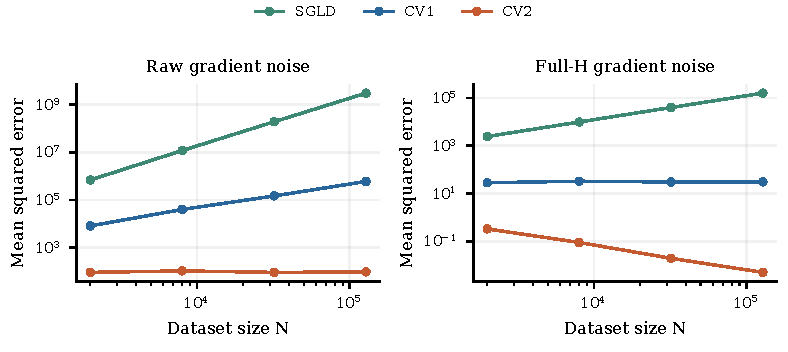
\includegraphics[width=\linewidth]{figures/noise_scaling.pdf}
\caption{Raw (left) and preconditioned (right) exact gradient-noise MSE against $N$ at fixed $n=16$, on one nested synthetic realization. All observations are enumerated at $32$ reference locations per size.}\label{fig:noise_scaling}
\end{figure}

\paragraph{Optimized time-to-accuracy.}
For each $N$, the same bounded pilot/selection rules choose independent validation candidates, without importing Bank-optimal parameters. There are $192$ pilot and $192$ validation runs per size, $1536$ in total. All validation runs are complete with no failures or censoring. We emphasize the cross-$N$ joint time-to-accuracy and speedup summary in the main text; the complete marginal frontier point clouds for each $N$ appear in Appendix~\ref{app:n_frontiers}. CV2 remains faster at the four representative accuracy targets (Table~\ref{tab:n_scaling}), but its speedup decreases between $N=2000$ and $128000$ by approximately $33\%,61\%,49\%,25\%$ for variance thresholds $0.5,0.4,0.3,0.2$. The trajectory across sizes need not be monotone, and CV2 is not faster at every one of the $41$ thresholds for every size. No eligible configuration at any size violates SW$_2\leq0.3$. At every size, CV2's selected configuration uses the smallest tested batch, $n=1$, at $40$ or $41$ of the $41$ warm thresholds, and also the earliest checkpoint, $K=128$, at $23$--$25$ of them; within this grid, further CV2 variance reduction cannot always be converted into saved work.
\begin{table}[tb]
\centering\small
\caption{Synthetic dataset-size scaling: setup-inclusive warm point-attainment speedup CV1/CV2, with whitened SW$_2\leq0.3$.}\label{tab:n_scaling}
\begin{tabular}{rrrrr}
\toprule
Variance & $N=2000$ & $8000$ & $32000$ & $128000$ \\
\midrule
0.50 & 2.146 & 2.137 & 1.825 & 1.441 \\
0.40 & 3.684 & 3.432 & 1.807 & 1.428 \\
0.30 & 4.326 & 4.762 & 2.845 & 2.210 \\
0.20 & 4.363 & 4.638 & 4.205 & 3.273 \\
\bottomrule
\end{tabular}
\par\smallskip{\footnotesize At variance threshold $0.3$, approximate 95\% intervals in increasing-$N$ order are $[3.438,4.391]$, $[4.260,5.362]$, $[2.830,2.860]$, $[2.141,2.259]$.}
\end{table}

\begin{figure}[tb]
\centering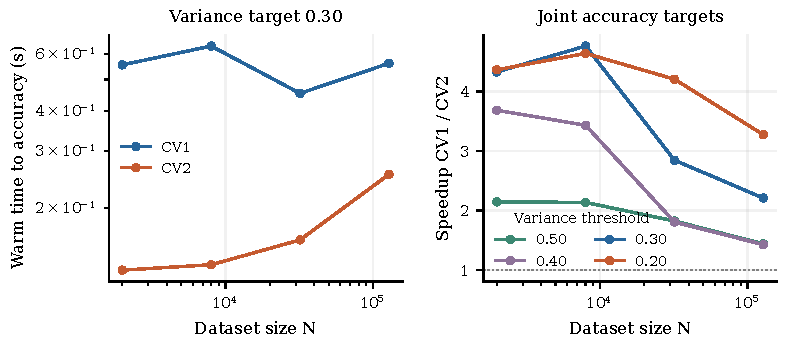
\includegraphics[width=\linewidth]{figures/n_efficiency.pdf}
\caption{Setup-inclusive warm point-attainment time-to-accuracy with independent tuning and validation at each $N$, requiring SW$_2\leq0.3$. Left: times at variance target $0.3$. Right: CV1/CV2 speedups at four variance targets.}\label{fig:n_efficiency}
\end{figure}

\paragraph{Why does total speedup decline?}
A saved-prefix cost decomposition, requiring no new sampling, writes $T_m=A_m+K_mc_m$, where $A_m$ is attributed setup and $c_m$ is batched sampling time per step. At variance threshold $0.5$, sampling-only speedup stays approximately $2.21$--$2.26$, while setup-inclusive speedup falls from $2.15$ to $1.44$. The noise advantage itself grows much faster than either time advantage: from $N=2000$ to $128000$, the CV1/CV2 ratio of reference-location gradient-noise MSE rises from about $89$ to $6270$ in raw terms and from about $86$ to $6190$ after preconditioning, roughly $70$-fold. Together with CV2's selections at the smallest tested batch and often the earliest checkpoint, this pattern is consistent with gradient noise no longer limiting CV2's accuracy, so that further variance reduction cannot be converted into additional saved work within the tested grid. CV2's setup share rises from $5.5\%$ to $65.0\%$: the common additive mode/metric preparation cost increasingly dilutes its already faster sampling. At stricter targets, CV1's changed batch, step and iteration choices also narrow the work gap. At matched configurations, CV2/CV1 per-step timing ratios range only from $0.982$ to $1.071$; there is no observed large growth of CV2-specific overhead sufficient to explain the total decline. This is an accounting decomposition and observational timing control, not randomized causal attribution (Appendix~\ref{app:cost}).

\FloatBarrier
\paragraph{Full-gradient ULA comparison.}\label{sec:exp_ula}
To assess whether CV2's measured benefits extend beyond comparisons with first-order control variates, we conducted a review-motivated, two-stage extension against full-gradient ULA at $N=2000$ and $N=128000$. Configurations were selected in an exploratory pilot and then evaluated without reselection on eight independent held-out seeds with $512$ mode-start replicas each. All $136$ validation runs completed without failed replicas or censoring. At $N=128000$, the simultaneous upper bounds for all three methods satisfy SW$_2\leq0.3$ and relative variance NRMSE$\leq0.3$. Under setup-inclusive warm accounting, CV2 reaches this joint target in $0.247$ seconds, compared with $0.560$ for CV1 and $16.3$ for ULA. The corresponding CV1/CV2 and ULA/CV2 time ratios are $2.26$ (approximate paired bootstrap 95\% interval $[2.19,2.34]$) and $65.9$ ($[62.7,69.8]$). From the same reported times, CV1 is itself about $29$ times faster than ULA, so most of the ULA/CV2 ratio reflects control-variate minibatching in general; the CV1/CV2 ratio isolates the additional contribution of the second-order correction. At $N=2000$, the point-estimate ULA/CV2 ratio is $4.21$, but CV2's simultaneous upper variance bound is $0.310$, above the $0.3$ tolerance; only $68.9\%$ of paired bootstrap draws jointly attain the target. This smaller-endpoint comparison is descriptive, rather than evidence of simultaneous-supported target attainment.

The pilot freezes a separate $(h,n,K)$ policy for each cost convention and tolerance; failure to attain a target refers to that preselected policy, not every tested configuration. Warm time includes attributed mode fitting and actual full-Hessian/cache preparation but excludes JIT compilation; cold time additionally attributes shape-specific compilation in the shared process. Thus the extension supports a substantial advantage over the selected ULA policy at the tested large-data endpoint, rather than a universal speedup or an independently reoptimized held-out frontier. \par\begin{samepage}
The advantage over full-gradient sampling is conditional: at $N=2000$ it is not supported at the simultaneous level, and on original Bank (Section~\ref{sec:exp_accuracy}) only ULA reached the frozen joint target in the selected-step comparison.
\par\end{samepage}

In summary, P3B provides the prospectively frozen efficiency evidence. CV2 reaches the four representative joint targets $1.43$--$4.76$ times faster than CV1 at every tested $N$, but the advantage narrows as $N$ grows, because shared setup takes a growing share of total time and CV2's additional noise reduction stops translating into saved work.

\FloatBarrier
\subsection{Mixing efficiency and computational cost}\label{sec:exp_ess}
Sections~\ref{sec:exp_accuracy}--\ref{sec:exp_scaling} measure accuracy at fixed budgets or time to a joint accuracy target. This subsection adds a descriptive chain-efficiency summary from existing post-burn-in records. For seed $s$, let $E_s$ be the smallest coordinate bulk ESS over $C$ unthinned chains, each with $T$ retained draws after $B$ burn-in transitions. We report $E_s$ per setup-inclusive second and per counted observation-gradient call, as medians of per-seed ratios. A configuration is eligible only if every seed passes maximum rank-$\widehat R<1.01$ and minimum coordinate bulk and tail ESS of at least $400$, with no numerical failure and a fixed metric.

Table~\ref{tab:german_ess} compares CV1, CV2 and ULA at common full-H step $h=0.4$ on four German selection-stage seeds. CV2 has a similar minimum bulk ESS to CV1 ($3304$ versus $3262$), but lower setup-inclusive ESS per second ($4173$ versus $4597$); ESS per observation-gradient call is comparable. ULA's ESS per observation-gradient call is about $30$ times lower, because each of its steps uses all $1000$ observations, while its ESS per second remains within about $25\%$ of CV1's on this small dataset. Observation-gradient counts exclude Hessian work, which enters measured time; Hessian contributions and data-row visits are separate operation units, and we do not convert them into gradient equivalents.

These NumPy CPU diagnostics assess chain mixing, not posterior approximation accuracy, and do not form an optimized time-to-accuracy comparison; passing the mixing gate does not remove discretization bias. The principal P1--P3 endpoint and running-functional archives do not record within-chain autocorrelation, so comparable ESS is not available for the optimized studies. Appendix~\ref{app:ess_cost} lists all eight eligible configuration groups, including historical YearMSD settings with unequal chain budgets, and all $39$ excluded groups, among them identity SGLD and the adaptive controls.

\begin{table}[!htbp]
\centering\small
\caption{German Credit post-burn-in mixing diagnostics at fixed full-H $h=0.4$. Each displayed configuration passes all four selection-stage seeds; entries are medians across those seeds.}\label{tab:german_ess}
\setlength{\tabcolsep}{4pt}
\begin{tabular}{lrrr}
\toprule
Method & Min bulk ESS & ESS/s & ESS/obs. grad. \\
\midrule
CV1 & 3262.1 & 4596.9 & 0.004943 \\
CV2 & 3303.6 & 4172.5 & 0.005005 \\
ULA & 3304.9 & 3515.7 & 0.000165 \\
\bottomrule
\end{tabular}
\par\smallskip{\footnotesize Each seed uses four chains, $1000$ discarded burn-in transitions and $4000$ retained draws per chain. CV1/CV2 use batch $32$; ULA uses all $1000$ observations. The numerator is the smallest coordinate bulk ESS within each seed. Ratios are formed per seed before taking medians. Seconds include setup and burn-in; gradient counts exclude Hessian work, which is included in measured time.}
\end{table}

\FloatBarrier
\subsection{Gaussian verification (P4)}\label{sec:exp_gaussian}
A focused quadratic finite-sum check uses $N=256,d=10$, condition numbers $10$ and $10^4$, identity/full-H metrics, four paired seeds and $512$ replicas. CV2 explicitly evaluates the minibatch Taylor remainder. Across $32$ fixed-budget method runs, its maximum scaled gradient discrepancy from the full gradient is $3.54\times10^{-13}$ and its maximum whitened path discrepancy from ULA, under shared initialization and Gaussian innovations, is $4.62\times10^{-13}$. All numerical gates pass, with no failures.

Exact finite-step Gaussian laws isolate geometry and discretization. At $K=1024$ and $\kappa=10^4$, population $W_2$ is $2.604$ under identity versus $0.0822$ under full-H. At $\kappa=10$, the corresponding values are $0.0194$ and $0.0822$: full-H removes slow geometry but need not minimize final error under the common stability-coefficient rule. It retains discretization bias, and mode-start transient discrepancy can be nonmonotone. Empirical full optimal-transport distances and independent exact-vs-exact baselines are reported separately from these analytic population distances. No speedup conclusion is drawn from this verification (Appendix~\ref{app:gaussian}).

A historical YearPredictionMSD Gaussian-ridge study supplies a complementary real-data example: near-exact CV2 gradients do not overcome severely ill-conditioned identity geometry, whereas full-H arms pass the declared mixing checks. Appendix~\ref{app:year_geometry} preserves its chain-based evaluation, direct Gaussian control and limitations separately from the independent-replica efficiency studies.

\subsection{Experimental discussion}\label{sec:exp_discussion}
The experiments address three successive questions. First, does CV2 reduce stochastic-gradient noise as intended? In the nested synthetic family it does: raw and preconditioned noise-scaling slopes agree qualitatively with the predicted orders (Section~\ref{sec:exp_scaling}). Second, does that reduction save computation at matched accuracy? Under prospectively frozen tuning and validation, CV2 reaches the four representative joint targets $1.43$--$4.76$ times faster than CV1 at every tested $N$, and at $N=128000$ it is also substantially faster than the selected full-gradient ULA policy. On the transformed Bank target, validated speedups are $2.27$--$6.27$. Third, when does the benefit fail to appear?

Three conditions emerge. First, stochastic-gradient noise must materially limit the chosen posterior accuracy: variance reduction has little measurable time value when discretization or a loose target dominates, as in the P2 synthetic targets, where every method meets the original loose target at the earliest checkpoint, and in P3B, where a roughly $70$-fold growth in the noise ratio leaves sampling-only speedup at variance threshold $0.5$ near $2.2$. Second, the observation-level remainder distribution must permit useful stable steps; global whitening does not remove every high-leverage contribution, as the original Bank failures show. Third, saved sampling work must outweigh preparation and competing-method retuning, which explains the declining setup-inclusive speedup in P3B. These conditions explain why the strongest computational evidence comes from independently validated optimized P3 comparisons, while P1/P2 and the original Bank results retain important null or unfavorable findings.

Posterior geometry is a prerequisite rather than a source of CV2's relative advantage in these experiments. All main comparisons share one fixed full-Hessian metric, and P4 and the YearMSD study show that exact gradients alone do not overcome ill-conditioned identity geometry. Overall, under a fixed geometry-correcting preconditioner, second-order control variates can translate improved stochastic-gradient precision into substantial time-to-accuracy savings, but only when gradient noise limits accuracy; rare high-leverage Taylor remainders and shared setup costs can erase or dilute the benefit. The experiments therefore support a conditional accuracy--cost benefit, rather than uniform superiority over first-order control variates.

\subsection{Scope and limitations}\label{sec:exp_limitations}
The following conditions apply throughout this section. References are approximate Metropolis-corrected HMC draws; passing the reference diagnostic gates is necessary for the reported rankings but does not prove an exact reference distribution. SW$_2$ is a finite-cloud projected discrepancy rather than certified population $W_2$, and finite-cloud reference-versus-reference discrepancies are reported but not subtracted as a bias correction. Bootstrap intervals use eight algorithm-seed clusters and condition on fixed references; simultaneous accuracy bands are approximately calibrated within their declared family and carry no joint guarantee across dataset sizes.

All optima are restricted to frozen, finite candidate grids. Minima selected among validation candidates remain potentially optimistic. The $41$ variance thresholds are strongly dependent rather than separate tests, and configuration changes between adjacent thresholds can make speedup curves nonmonotone. Absolute times depend on hardware and implementation: NumPy CPU, A100/T4 GPU and JAX CPU sessions, including the new ULA measurements, are not pooled into one ranking. Production minibatches in P1--P3 are drawn without replacement and use the fixed metric~\eqref{eq:exp_update} (Appendix~\ref{app:metrics}). Passing a chain mixing gate does not imply posterior accuracy. The P3A evidence concerns a transformed posterior whose transformation and tuning were both chosen after the original results, and the dataset-size study uses one nested Gaussian-design realization.
